\begin{figure}[H]
  \centering
  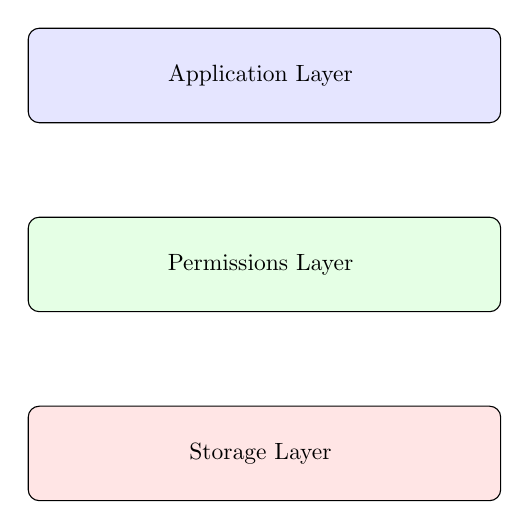
\begin{tikzpicture}[scale = 0.6, every node/.style={scale = 0.85}, every node/.append style={fill = white, rounded corners = 2pt, inner sep = 2pt, align = center}]
  
  % Layer boxes
  \draw [rounded corners, fill=blue!10] (-5, 5) rectangle (5, 3);
  \node [fill=blue!10] at (0, 4) { Application Layer };
  
  
  
  \draw [rounded corners, fill=green!10] (-5, 1) rectangle (5, -1);
  \node [fill=green!10] at (0, 0) { Permissions Layer };
  
  
  
  \draw [rounded corners, fill=red!10] (-5, -5) rectangle (5, -3);
  \node [fill=red!10] at (0, -4) { Storage Layer };
  
  \end{tikzpicture} \\
  \caption{
  	Platform Layer Communication (Centralised)
  }
  \label{fig:archi_platform_layers_centralised}
\end{figure}